\cajita{Número de casos de mujeres embarazadas entre 10 y 54 años atendidas por el sistema de salud pública}{La tabla muestra el número de mujeres embarazadas entre 10 y 54 años atendidas por el sistema de salud pública de 2018 al 2022. 

En 2018 el grupo de edad con mayor número de casos fue de 20 a 24 años con 262,659 casos y el cual disminuyó 110,587 casos en 2021.


}{Número de casos de mujeres embarazadas entre 10 y 54 años atendidas por el sistema de salud pública, 2018 - 2021}{República de Guatemala, Instituto Nacional de Estadística}{\\[-0.5cm]\begin{tabular}[t]{ccccc}
\toprule
\textbf{Grupos de edad} & \textbf{2018} & \textbf{2019} & \textbf{2020} & \textbf{2021}\\
\midrule
\cellcolor[HTML]{B6B3FF}{10-14} & \cellcolor[HTML]{B6B3FF}{7,506} & \cellcolor[HTML]{B6B3FF}{7,659} & \cellcolor[HTML]{B6B3FF}{6,856} & \cellcolor[HTML]{B6B3FF}{4,703}\\
15-19 & 213,959 & 208,480 & 172,575 & 109,175\\
\cellcolor[HTML]{B6B3FF}{20-24} & \cellcolor[HTML]{B6B3FF}{262,659} & \cellcolor[HTML]{B6B3FF}{267,762} & \cellcolor[HTML]{B6B3FF}{230,079} & \cellcolor[HTML]{B6B3FF}{152,072}\\
25-29 & 172,892 & 179,403 & 157,491 & 105,699\\
\cellcolor[HTML]{B6B3FF}{30-34} & \cellcolor[HTML]{B6B3FF}{103,730} & \cellcolor[HTML]{B6B3FF}{106,045} & \cellcolor[HTML]{B6B3FF}{92,247} & \cellcolor[HTML]{B6B3FF}{62,014}\\
35-39 & 54,894 & 55,248 & 48,358 & 31,769\\
\cellcolor[HTML]{B6B3FF}{40-44} & \cellcolor[HTML]{B6B3FF}{15,872} & \cellcolor[HTML]{B6B3FF}{15,848} & \cellcolor[HTML]{B6B3FF}{13,716} & \cellcolor[HTML]{B6B3FF}{9,198}\\
45-49 & 1,375 & 1,462 & 1,099 & 655\\
\cellcolor[HTML]{B6B3FF}{50-54} & \cellcolor[HTML]{B6B3FF}{258} & \cellcolor[HTML]{B6B3FF}{263} & \cellcolor[HTML]{B6B3FF}{198} & \cellcolor[HTML]{B6B3FF}{132}\\
\bottomrule
\end{tabular}
}{INE - MSPAS - SIGSA, 2023}{}

\cajita{Métodos de planificación familiar entregados por el sistema de salud pública por sexo}{La tabla muestra la cantidad de métodos de planificación familiar entregados por el sistema de salud pública por sexo, según el tipo de usuarios.

Para 2018 se entregó una total de 1,638,468 de métodos de planificación familiar a mujeres y hombres usuarios del sistema de salud pública. Se atendieron a 1,041,018 mujeres en reconsulta y a 575,437 mujeres en primera consulta. 

Para 2022 se entregó una total de 1,161,566 de métodos de planificación familiar a mujeres y hombres usuarios del sistema de salud pública. De estos se atendieron a 604,890 mujeres en reconsulta y 530,699 mujeres en primera consulta. 
}{Métodos de planificación familiar entregados por el sistema de salud pública por sexo, 2018 - 2022}{República de Guatemala, Instituto Nacional de Estadística}{\\[-0.5cm]\begin{tabular}[t]{ccccc}
\toprule
\multicolumn{1}{c}{\textbf{ }} & \multicolumn{2}{c}{\textbf{Usuarios nuevos}} & \multicolumn{2}{c}{\textbf{Usuarios reconsultas}} \\
\cmidrule(l{3pt}r{3pt}){2-3} \cmidrule(l{3pt}r{3pt}){4-5}
\textbf{Año} & \textbf{Mujeres} & \textbf{Hombres} & \textbf{Mujeres} & \textbf{Hombres}\\
\midrule
\cellcolor[HTML]{B6B3FF}{2018} & \cellcolor[HTML]{B6B3FF}{575,437} & \cellcolor[HTML]{B6B3FF}{14,132} & \cellcolor[HTML]{B6B3FF}{1,041,018} & \cellcolor[HTML]{B6B3FF}{7,881}\\
2019 & 567,097 & 16,917 & 1,042,881 & 9,698\\
\cellcolor[HTML]{B6B3FF}{2020} & \cellcolor[HTML]{B6B3FF}{534,339} & \cellcolor[HTML]{B6B3FF}{15,679} & \cellcolor[HTML]{B6B3FF}{970,926} & \cellcolor[HTML]{B6B3FF}{9,903}\\
2021 & 515,108 & 17,534 & 804,710 & 10,306\\
\cellcolor[HTML]{B6B3FF}{2022} & \cellcolor[HTML]{B6B3FF}{530,699} & \cellcolor[HTML]{B6B3FF}{15,551} & \cellcolor[HTML]{B6B3FF}{604,890} & \cellcolor[HTML]{B6B3FF}{10,426}\\
\bottomrule
\end{tabular}
}{INE - MSPAS - SIGSA, 2023}{}

\cajita{Métodos de planificación familiar entregados por sexo, según tipo de método}{La tabla muestra la cantidad de métodos de planificación familiar entregados a usuarios del sistema de salud pública por sexo, según tipo de método de planficación durante el 2022. 

Los datos no reflejan el total de métodos de planifiación familiar que usaron mujeres y hombres, estos son métodos entregados a usuarios del sistema de salud en primera consulta y en reconsulta. 

Los métodos de planificación familiar como el inyectable, DIU, píldora e implante subdérmico son métodos entregado únicamente a mujeres. A diferencia de los métodos de barrera y quírurgico que son entregados a hombres y mujeres. }{Métodos de planificación familiar entregados por sexo, según tipo de método, 2022}{República de Guatemala, Instituto Nacional de Estadística}{\\[-0.5cm]\begin{tabular}[t]{ccc}
\toprule
\textbf{Tipo de Método} & \textbf{Mujeres} & \textbf{Hombres}\\
\midrule
\cellcolor[HTML]{B6B3FF}{Barrera} & \cellcolor[HTML]{B6B3FF}{48262} & \cellcolor[HTML]{B6B3FF}{25811}\\
Inyectable & 938482 & NA\\
\cellcolor[HTML]{B6B3FF}{DIU} & \cellcolor[HTML]{B6B3FF}{5100} & \cellcolor[HTML]{B6B3FF}{NA}\\
Píldora & 58250 & NA\\
\cellcolor[HTML]{B6B3FF}{Implante subdérmico} & \cellcolor[HTML]{B6B3FF}{32172} & \cellcolor[HTML]{B6B3FF}{NA}\\
Natural & 48796 & 0\\
\cellcolor[HTML]{B6B3FF}{Quirúrgico} & \cellcolor[HTML]{B6B3FF}{4527} & \cellcolor[HTML]{B6B3FF}{166}\\
\bottomrule
\end{tabular}
}{INE - MSPAS - SIGSA, 2023}{}
\\[-0.5cm]
\cajita{Nacimientos por edad de la madre, según grupos de edad}{La tabla muestra el número de nacimientos registrados por edad de la madre del 2018 a 2021. 

En el 2018 y 2021 el grupo de edad con más nacimientos registrados fue el de 20 a 24 años con 117,125 casos en el 2018 y 105,003 casos en el 2021. Seguido del 25 a 29 años con 89,425 en el 2018 y 83,683 en el 2021.   }{Nacimientos por edad de la madre, según grupos de edad (número de casos), 2018 - 2021}{República de Guatemala, Instituto Nacional de Estadística}{\\[-0.5cm]\begin{tabular}[t]{ccccc}
\toprule
\textbf{Grupos de edad} & \textbf{2018} & \textbf{2019} & \textbf{2020} & \textbf{2021}\\
\midrule
\cellcolor[HTML]{B6B3FF}{Menos de 15} & \cellcolor[HTML]{B6B3FF}{2004} & \cellcolor[HTML]{B6B3FF}{1914} & \cellcolor[HTML]{B6B3FF}{1578} & \cellcolor[HTML]{B6B3FF}{1805}\\
15 - 19 & 72615 & 67984 & 60410 & 60731\\
\cellcolor[HTML]{B6B3FF}{20 - 24} & \cellcolor[HTML]{B6B3FF}{117125} & \cellcolor[HTML]{B6B3FF}{112059} & \cellcolor[HTML]{B6B3FF}{105610} & \cellcolor[HTML]{B6B3FF}{105003}\\
25 - 29 & 89425 & 87019 & 82401 & 83683\\
\cellcolor[HTML]{B6B3FF}{30 - 34} & \cellcolor[HTML]{B6B3FF}{59125} & \cellcolor[HTML]{B6B3FF}{57213} & \cellcolor[HTML]{B6B3FF}{53221} & \cellcolor[HTML]{B6B3FF}{54809}\\
35 - 39 & 32409 & 30783 & 28846 & 29583\\
\cellcolor[HTML]{B6B3FF}{40 - 44} & \cellcolor[HTML]{B6B3FF}{9744} & \cellcolor[HTML]{B6B3FF}{9161} & \cellcolor[HTML]{B6B3FF}{8513} & \cellcolor[HTML]{B6B3FF}{8840}\\
45 - 49 & 633 & 594 & 521 & 577\\
\cellcolor[HTML]{B6B3FF}{50 y más} & \cellcolor[HTML]{B6B3FF}{44} & \cellcolor[HTML]{B6B3FF}{36} & \cellcolor[HTML]{B6B3FF}{31} & \cellcolor[HTML]{B6B3FF}{36}\\
Ignorado & 139 & 92 & 81 & 82\\
\bottomrule
\end{tabular}
}{INE - Estadísticas Vitales 2022}{} %4

\cajita{Partos atendidos por tipo de asistencia}{La tabla muestra el porcentaje de partos atendidos según el tipo de asistencia del 2018 al 2021. 

En el 2018 del total de partos la asistencia médica fue de 71.6\% y para el 2021 fue de 68.8\%. La asistencia atendida por comadrona para el 2018 fue de 26.6\% y para el 2021 fue de 26.5\%. La asistencia empírica en el 2018 fue de 0.3\%  y para el 2021 fue de 1.0\%. }{Porcentaje de partos atendidos por tipo de asistencia (porcentaje) 2018-2021}{República de Guatemala, Instituto Nacional de Estadística}{\\[-0.5cm]\begin{tabular}[t]{ccccc}
\toprule
\textbf{Tipo de Asistencia} & \textbf{2018} & \textbf{2019} & \textbf{2020} & \textbf{2021}\\
\midrule
\cellcolor[HTML]{B6B3FF}{Médica} & \cellcolor[HTML]{B6B3FF}{71.6} & \cellcolor[HTML]{B6B3FF}{73.8} & \cellcolor[HTML]{B6B3FF}{68.9} & \cellcolor[HTML]{B6B3FF}{68.8}\\
Paramédica & 0.4 & 0.3 & 0.3 & 0.3\\
\cellcolor[HTML]{B6B3FF}{Comadrona} & \cellcolor[HTML]{B6B3FF}{26.6} & \cellcolor[HTML]{B6B3FF}{23.5} & \cellcolor[HTML]{B6B3FF}{26.6} & \cellcolor[HTML]{B6B3FF}{26.5}\\
Empírica & 0.3 & 0.8 & 1.0 & 1.0\\
\cellcolor[HTML]{B6B3FF}{Ninguna} & \cellcolor[HTML]{B6B3FF}{0.1} & \cellcolor[HTML]{B6B3FF}{0.3} & \cellcolor[HTML]{B6B3FF}{0.4} & \cellcolor[HTML]{B6B3FF}{0.4}\\
Ignorado & 1.0 & 1.3 & 2.9 & 2.9\\
\bottomrule
\end{tabular}
}{INE - Estadísticas Vitales, 2022}{} %5
\\[-1.5cm]
\cajita{Personas notificadas con VIH/SIDA por sexo}{La gráfica muestra el porcentaje de mujeres y hombres notificados con VIH/SIDA del 2018 al 2022. 

En el 2018 del total de casos reportados el 35.9\% eran mujeres, en el 2022 del total de casos reportados el 28.9\% eran mujeres. }{Personas notificadas con VIH/SIDA por sexo (porcentaje), 2018-2022}{República de Guatemala, Instituto Nacional de Estadística }{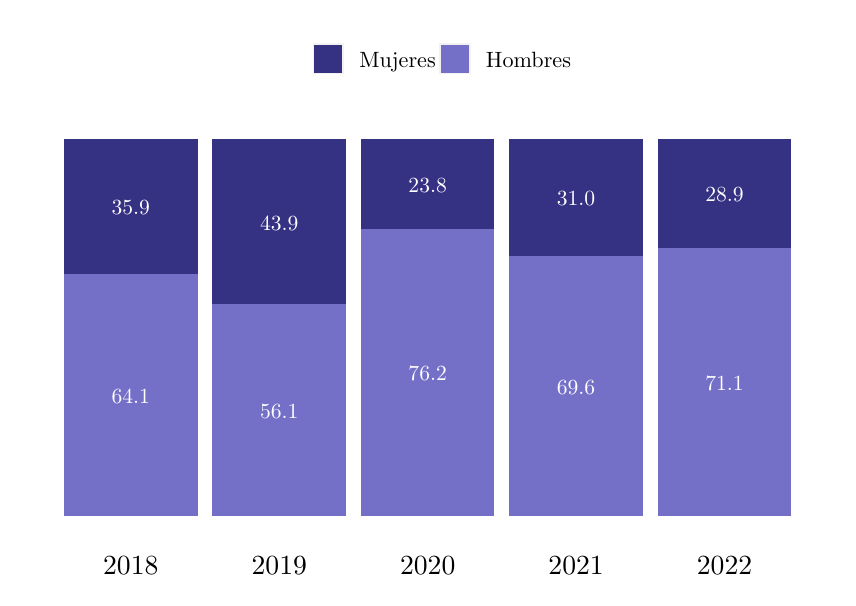
\begin{tikzpicture}[x=1pt,y=1pt]% Created by tikzDevice version 0.12.4 on 2023-05-15 15:42:39
% !TEX encoding = UTF-8 Unicode
\definecolor{fillColor}{RGB}{255,255,255}
\path[use as bounding box,fill=fillColor,fill opacity=0.00] (0,0) rectangle (289.08,198.74);
\begin{scope}
\path[clip] (  0.00,  0.00) rectangle (289.08,198.74);

\path[] (  0.00,  0.00) rectangle (289.08,198.74);
\end{scope}
\begin{scope}
\path[clip] (  0.00,  0.00) rectangle (289.08,198.74);
\definecolor{fillColor}{RGB}{54,50,131}

\path[fill=fillColor] ( 13.14,109.64) rectangle ( 61.41,158.54);

\path[fill=fillColor] ( 66.77, 98.71) rectangle (115.04,158.54);

\path[fill=fillColor] (120.41,126.08) rectangle (168.67,158.54);

\path[fill=fillColor] (174.04,116.28) rectangle (222.31,158.54);

\path[fill=fillColor] (227.67,119.21) rectangle (275.94,158.54);
\definecolor{fillColor}{RGB}{116,112,200}

\path[fill=fillColor] ( 13.14, 22.21) rectangle ( 61.41,109.64);

\path[fill=fillColor] ( 66.77, 22.21) rectangle (115.04, 98.71);

\path[fill=fillColor] (120.41, 22.21) rectangle (168.67,126.08);

\path[fill=fillColor] (174.04, 22.21) rectangle (222.31,116.28);

\path[fill=fillColor] (227.67, 22.21) rectangle (275.94,119.21);
\definecolor{drawColor}{RGB}{255,255,255}

\node[text=drawColor,anchor=base,inner sep=0pt, outer sep=0pt, scale=  0.78] at ( 37.27,131.06) {35.9};

\node[text=drawColor,anchor=base,inner sep=0pt, outer sep=0pt, scale=  0.78] at ( 90.91,125.59) {43.9};

\node[text=drawColor,anchor=base,inner sep=0pt, outer sep=0pt, scale=  0.78] at (144.54,139.28) {23.8};

\node[text=drawColor,anchor=base,inner sep=0pt, outer sep=0pt, scale=  0.78] at (198.17,134.38) {31.0};

\node[text=drawColor,anchor=base,inner sep=0pt, outer sep=0pt, scale=  0.78] at (251.81,135.85) {28.9};

\node[text=drawColor,anchor=base,inner sep=0pt, outer sep=0pt, scale=  0.78] at ( 37.27, 62.89) {64.1};

\node[text=drawColor,anchor=base,inner sep=0pt, outer sep=0pt, scale=  0.78] at ( 90.91, 57.43) {56.1};

\node[text=drawColor,anchor=base,inner sep=0pt, outer sep=0pt, scale=  0.78] at (144.54, 71.11) {76.2};

\node[text=drawColor,anchor=base,inner sep=0pt, outer sep=0pt, scale=  0.78] at (198.17, 66.22) {69.6};

\node[text=drawColor,anchor=base,inner sep=0pt, outer sep=0pt, scale=  0.78] at (251.81, 67.68) {71.1};

\path[] (  0.00, 15.40) rectangle (289.08,165.36);
\end{scope}
\begin{scope}
\path[clip] (  0.00,  0.00) rectangle (289.08,198.74);

\path[] (  0.00, 15.40) --
	(  0.00,165.36);
\end{scope}
\begin{scope}
\path[clip] (  0.00,  0.00) rectangle (289.08,198.74);

\path[] (  0.00, 15.40) --
	(289.08, 15.40);
\end{scope}
\begin{scope}
\path[clip] (  0.00,  0.00) rectangle (289.08,198.74);

\path[] ( 37.27, 12.65) --
	( 37.27, 15.40);

\path[] ( 90.91, 12.65) --
	( 90.91, 15.40);

\path[] (144.54, 12.65) --
	(144.54, 15.40);

\path[] (198.17, 12.65) --
	(198.17, 15.40);

\path[] (251.81, 12.65) --
	(251.81, 15.40);
\end{scope}
\begin{scope}
\path[clip] (  0.00,  0.00) rectangle (289.08,198.74);
\definecolor{drawColor}{RGB}{0,0,0}

\node[text=drawColor,anchor=base,inner sep=0pt, outer sep=0pt, scale=  1.00] at ( 37.27,  1.32) {2018};

\node[text=drawColor,anchor=base,inner sep=0pt, outer sep=0pt, scale=  1.00] at ( 90.91,  1.32) {2019};

\node[text=drawColor,anchor=base,inner sep=0pt, outer sep=0pt, scale=  1.00] at (144.54,  1.32) {2020};

\node[text=drawColor,anchor=base,inner sep=0pt, outer sep=0pt, scale=  1.00] at (198.17,  1.32) {2021};

\node[text=drawColor,anchor=base,inner sep=0pt, outer sep=0pt, scale=  1.00] at (251.81,  1.32) {2022};
\end{scope}
\begin{scope}
\path[clip] (  0.00,  0.00) rectangle (289.08,198.74);
\definecolor{fillColor}{RGB}{255,255,255}

\path[fill=fillColor] ( 91.98,176.36) rectangle (197.10,198.74);
\end{scope}
\begin{scope}
\path[clip] (  0.00,  0.00) rectangle (289.08,198.74);
\definecolor{fillColor}{gray}{0.95}

\path[fill=fillColor] (102.98,181.86) rectangle (114.36,193.24);
\end{scope}
\begin{scope}
\path[clip] (  0.00,  0.00) rectangle (289.08,198.74);
\definecolor{fillColor}{RGB}{54,50,131}

\path[fill=fillColor] (103.64,182.52) rectangle (113.70,192.58);
\end{scope}
\begin{scope}
\path[clip] (  0.00,  0.00) rectangle (289.08,198.74);
\definecolor{fillColor}{gray}{0.95}

\path[fill=fillColor] (148.72,181.86) rectangle (160.10,193.24);
\end{scope}
\begin{scope}
\path[clip] (  0.00,  0.00) rectangle (289.08,198.74);
\definecolor{fillColor}{RGB}{116,112,200}

\path[fill=fillColor] (149.38,182.52) rectangle (159.43,192.58);
\end{scope}
\begin{scope}
\path[clip] (  0.00,  0.00) rectangle (289.08,198.74);
\definecolor{drawColor}{RGB}{0,0,0}

\node[text=drawColor,anchor=base west,inner sep=0pt, outer sep=0pt, scale=  0.80] at (119.86,184.43) {Mujeres};
\end{scope}
\begin{scope}
\path[clip] (  0.00,  0.00) rectangle (289.08,198.74);
\definecolor{drawColor}{RGB}{0,0,0}

\node[text=drawColor,anchor=base west,inner sep=0pt, outer sep=0pt, scale=  0.80] at (165.60,184.43) {Hombres};
\end{scope}
\end{tikzpicture}}{MSPAS - SIGSA, 2023}{} %6

\cajita{Número de casos de mujeres seropositivas embarazadas entre 15 y 49 años por Pueblo}{La tabla muestra el número de casos de mujeres seropositivas embarazadas por pueblo de 2018 a 2022.  

En 2018 se reportó 112 casos en mujeres ladinas y 68 casos en mujeres mayas. En 2022 se reportó 83 casos en mujeres ladinas y 20 casos en mujeres mayas. 

En 2020 y 2021 se reportó 4 casos de mujeres ladinas menores de 15 años y 2 casos en mujeres mayas menores de 15 años. }{Número de casos de mujeres seropositivas embarazadas entre 15 y 49 años por Pueblo, 2018-2021}{República de Guatemala, Instituto Nacional de Estadística}{\\[-0.5cm]\begin{tabular}[t]{cccccc}
\toprule
\textbf{Pueblos} & \textbf{2018} & \textbf{2019} & \textbf{2020} & \textbf{2021} & \textbf{2022}\\
\midrule
\cellcolor[HTML]{B6B3FF}{Ladinas} & \cellcolor[HTML]{B6B3FF}{112} & \cellcolor[HTML]{B6B3FF}{123} & \cellcolor[HTML]{B6B3FF}{111} & \cellcolor[HTML]{B6B3FF}{105} & \cellcolor[HTML]{B6B3FF}{83}\\
Mayas & 68 & 51 & 35 & 30 & 20\\
\cellcolor[HTML]{B6B3FF}{Xincas} & \cellcolor[HTML]{B6B3FF}{0} & \cellcolor[HTML]{B6B3FF}{0} & \cellcolor[HTML]{B6B3FF}{0} & \cellcolor[HTML]{B6B3FF}{0} & \cellcolor[HTML]{B6B3FF}{0}\\
Garífunas & 0 & 0 & 0 & 1 & 0\\
\cellcolor[HTML]{B6B3FF}{Otros} & \cellcolor[HTML]{B6B3FF}{0} & \cellcolor[HTML]{B6B3FF}{0} & \cellcolor[HTML]{B6B3FF}{0} & \cellcolor[HTML]{B6B3FF}{0} & \cellcolor[HTML]{B6B3FF}{0}\\
\bottomrule
\end{tabular}
}{MSPAS - SIGSA, 2023}{}
\\[-1.5cm]
\cajita{Tasa de mortalidad materna}{La gráfica muestra la tasa de mortalidad materna del 2018 a 2021. En 2021 la tasa de mortalidad materna fue 0.84, en 2020 de 0.76, en el 2019 de 0.67 y en 2018 de 0.76. }{Tasa de mortalidad materna, 2018-2021}{República de Guatemala, Instituto Nacional de Estadística}{\begin{tikzpicture}[x=1pt,y=1pt]% Created by tikzDevice version 0.12.4 on 2023-05-15 15:54:39
% !TEX encoding = UTF-8 Unicode
\definecolor{fillColor}{RGB}{255,255,255}
\path[use as bounding box,fill=fillColor,fill opacity=0.00] (0,0) rectangle (289.08,198.74);
\begin{scope}
\path[clip] (  0.00,  0.00) rectangle (289.08,198.74);

\path[] (  0.00,  0.00) rectangle (289.08,198.74);
\end{scope}
\begin{scope}
\path[clip] (  0.00,  0.00) rectangle (289.08,198.74);
\definecolor{drawColor}{RGB}{54,50,131}

\path[draw=drawColor,line width= 1.7pt,line join=round] ( 48.88, 84.13) --
	(113.23, 46.81) --
	(177.58, 82.98) --
	(241.93,116.14);
\definecolor{drawColor}{RGB}{0,0,0}

\node[text=drawColor,anchor=base,inner sep=0pt, outer sep=0pt, scale=  1.02] at ( 48.88, 88.10) {0.76};

\node[text=drawColor,anchor=base,inner sep=0pt, outer sep=0pt, scale=  1.02] at (113.23, 34.90) {0.67};

\node[text=drawColor,anchor=base east,inner sep=0pt, outer sep=0pt, scale=  1.02] at (174.46, 82.98) {0.76};

\node[text=drawColor,anchor=base,inner sep=0pt, outer sep=0pt, scale=  1.02] at (241.93,120.11) {0.84};

\path[draw=drawColor,line width= 0.1pt,line join=round] (-260.00, 26.01) -- (550.81, 26.01);

\path[] ( 10.27, 18.24) rectangle (280.54,189.21);

\path[] ( 10.27, 38.41) --
	(280.54, 38.41);

\path[] ( 10.27, 79.28) --
	(280.54, 79.28);

\path[] ( 10.27,120.14) --
	(280.54,120.14);

\path[] ( 10.27,161.01) --
	(280.54,161.01);

\path[] ( 10.27, 58.84) --
	(280.54, 58.84);

\path[] ( 10.27, 99.71) --
	(280.54, 99.71);

\path[] ( 10.27,140.58) --
	(280.54,140.58);

\path[] ( 10.27,181.44) --
	(280.54,181.44);

\path[] ( 48.88, 18.24) --
	( 48.88,189.21);

\path[] (113.23, 18.24) --
	(113.23,189.21);

\path[] (177.58, 18.24) --
	(177.58,189.21);

\path[] (241.93, 18.24) --
	(241.93,189.21);

\path[] ( 10.27, 18.24) rectangle (280.54,189.21);
\end{scope}
\begin{scope}
\path[clip] (  0.00,  0.00) rectangle (289.08,198.74);

\path[] ( 10.27, 18.24) --
	( 10.27,189.21);
\end{scope}
\begin{scope}
\path[clip] (  0.00,  0.00) rectangle (289.08,198.74);
\definecolor{drawColor}{RGB}{255,255,255}

\node[text=drawColor,text opacity=0.00,anchor=base east,inner sep=0pt, outer sep=0pt, scale=  1.00] at (  5.32, 54.93) {0.7};

\node[text=drawColor,text opacity=0.00,anchor=base east,inner sep=0pt, outer sep=0pt, scale=  1.00] at (  5.32, 95.80) {0.8};

\node[text=drawColor,text opacity=0.00,anchor=base east,inner sep=0pt, outer sep=0pt, scale=  1.00] at (  5.32,136.67) {0.9};

\node[text=drawColor,text opacity=0.00,anchor=base east,inner sep=0pt, outer sep=0pt, scale=  1.00] at (  5.32,177.53) {1.0};
\end{scope}
\begin{scope}
\path[clip] (  0.00,  0.00) rectangle (289.08,198.74);

\path[] (  7.52, 58.84) --
	( 10.27, 58.84);

\path[] (  7.52, 99.71) --
	( 10.27, 99.71);

\path[] (  7.52,140.58) --
	( 10.27,140.58);

\path[] (  7.52,181.44) --
	( 10.27,181.44);
\end{scope}
\begin{scope}
\path[clip] (  0.00,  0.00) rectangle (289.08,198.74);

\path[] ( 10.27, 18.24) --
	(280.54, 18.24);
\end{scope}
\begin{scope}
\path[clip] (  0.00,  0.00) rectangle (289.08,198.74);

\path[] ( 48.88, 15.49) --
	( 48.88, 18.24);

\path[] (113.23, 15.49) --
	(113.23, 18.24);

\path[] (177.58, 15.49) --
	(177.58, 18.24);

\path[] (241.93, 15.49) --
	(241.93, 18.24);
\end{scope}
\begin{scope}
\path[clip] (  0.00,  0.00) rectangle (289.08,198.74);
\definecolor{drawColor}{RGB}{0,0,0}

\node[text=drawColor,anchor=base,inner sep=0pt, outer sep=0pt, scale=  1.00] at ( 48.88,  4.16) {2018};

\node[text=drawColor,anchor=base,inner sep=0pt, outer sep=0pt, scale=  1.00] at (113.23,  4.16) {2019};

\node[text=drawColor,anchor=base,inner sep=0pt, outer sep=0pt, scale=  1.00] at (177.58,  4.16) {2020};

\node[text=drawColor,anchor=base,inner sep=0pt, outer sep=0pt, scale=  1.00] at (241.93,  4.16) {2021};
\end{scope}
\end{tikzpicture}}{INE - Estadísticas Vitales, 2022}{} % Esta pendiente verficar la tasa 

\cajota{Número de casos mortalidad materna según causa de muerte}{La tabla muertra el registro de defunciones de mujeres embarazas según la causa de muerte mas común de muerte. 

Para el 2018 las cassa de muerte mas común fue "complicaciones en el trabajo de parto y del parto" con 117 casos. En el 2021 la causa de muerte mas comun fue "Otras afecciones obstétricas no clasificadas en otra parte" con 105 casos reportardos. }{Número de casos mortalidad materna según causa de muerte, 2018 - 2021}{República de Guatemala, Instituto Nacional de Estadística}{\\[-1.5cm]\begin{tabular}[t]{ccccc}
\toprule
\textbf{Causas de Muerte} & \textbf{2018} & \textbf{2019} & \textbf{2020} & \textbf{2021}\\
\midrule
\cellcolor[HTML]{B6B3FF}{Embarazo terminado en aborto} & \cellcolor[HTML]{B6B3FF}{19} & \cellcolor[HTML]{B6B3FF}{23} & \cellcolor[HTML]{B6B3FF}{10} & \cellcolor[HTML]{B6B3FF}{14}\\
Hipertensión en el embarazo, el parto y el puerperio & 72 & 39 & 63 & 53\\
\cellcolor[HTML]{B6B3FF}{Otros trastornos maternos} & \cellcolor[HTML]{B6B3FF}{8} & \cellcolor[HTML]{B6B3FF}{6} & \cellcolor[HTML]{B6B3FF}{12} & \cellcolor[HTML]{B6B3FF}{9}\\
Atención materna relacionada con el feto & 21 & 27 & 15 & 14\\
\cellcolor[HTML]{B6B3FF}{Complicaciones del trabajo de parto} & \cellcolor[HTML]{B6B3FF}{117} & \cellcolor[HTML]{B6B3FF}{103} & \cellcolor[HTML]{B6B3FF}{101} & \cellcolor[HTML]{B6B3FF}{83}\\
Complicaciones con el puerperio & 17 & 27 & 18 & 12\\
\cellcolor[HTML]{B6B3FF}{Otras afecciones obstétricas} & \cellcolor[HTML]{B6B3FF}{38} & \cellcolor[HTML]{B6B3FF}{21} & \cellcolor[HTML]{B6B3FF}{40} & \cellcolor[HTML]{B6B3FF}{105}\\
\bottomrule
\end{tabular}
}{INE - Estadísticas Vitales, 2022}{}%9  

\cajota{Defunciones de mujeres por Pueblo, según causa de muerte}{La tabla muestra el número de defunciones registradas en mujeres por pueblo de pertenencia, según causa de muerte. 

En 2021 las tres causas más comunes de muerte en mujeres ladinas fue de "SARS-CoV2/COVID-19" con 4,107 casos, seguido de 	"Síntomas, signos y hallazgos anormales clínicos y de laboratorio" con 3,742 casos de "Infarto agudo del miocardio" con 3,742 casos. "Otras causas" registró 10,227 casos. 

En 2021 las tres causas más comunes de muerte en mujeres mayas fue de "Síntomas, signos y hallazgos anormales clínicos y de laboratorio" con 2,862 casos, seguido de "Diabetes mellitus no especificada" con 1,494 casos y "Infarto agudo del miocardio" con 1,345 casos. "Otras causas" registro 5,689 casos.}{Defunciones de mujeres por Pueblo, según causa de muerte, 2021}{República de Guatemala, Instituto Nacional de Estadística}{\\[-1.5cm]\begin{tabular}[t]{ccccccc}
\toprule
\multicolumn{1}{c}{\textbf{ }} & \multicolumn{6}{c}{\textbf{Pueblo de pertenencia}} \\
\cmidrule(l{3pt}r{3pt}){2-7}
\textbf{Causa de Muerte} & \textbf{Maya} & \textbf{Garífuna} & \textbf{Xinca} & \textbf{Ladino} & \textbf{Otro} & \textbf{Ignorado}\\
\midrule
\cellcolor[HTML]{B6B3FF}{SARS-CoV2/COVID-19} & \cellcolor[HTML]{B6B3FF}{1048} & \cellcolor[HTML]{B6B3FF}{4} & \cellcolor[HTML]{B6B3FF}{4} & \cellcolor[HTML]{B6B3FF}{4107} & \cellcolor[HTML]{B6B3FF}{91} & \cellcolor[HTML]{B6B3FF}{352}\\
Infarto agudo del miocardio & 1345 & 1 & 1 & 3058 & 82 & 334\\
\cellcolor[HTML]{B6B3FF}{Diabetes mellitus, no especificada} & \cellcolor[HTML]{B6B3FF}{1494} & \cellcolor[HTML]{B6B3FF}{2} & \cellcolor[HTML]{B6B3FF}{7} & \cellcolor[HTML]{B6B3FF}{2785} & \cellcolor[HTML]{B6B3FF}{51} & \cellcolor[HTML]{B6B3FF}{232}\\
Neumonía, organismo no especificado & 757 & 0 & 0 & 647 & 21 & 428\\
\cellcolor[HTML]{B6B3FF}{Diabetes mellitus no insulinodependiente} & \cellcolor[HTML]{B6B3FF}{666} & \cellcolor[HTML]{B6B3FF}{1} & \cellcolor[HTML]{B6B3FF}{1} & \cellcolor[HTML]{B6B3FF}{1051} & \cellcolor[HTML]{B6B3FF}{22} & \cellcolor[HTML]{B6B3FF}{90}\\
Accidente vascular encefálico agudo & 381 & 1 & 3 & 708 & 13 & 73\\
\cellcolor[HTML]{B6B3FF}{Fibrosis y cirrosis del hígado} & \cellcolor[HTML]{B6B3FF}{396} & \cellcolor[HTML]{B6B3FF}{0} & \cellcolor[HTML]{B6B3FF}{2} & \cellcolor[HTML]{B6B3FF}{617} & \cellcolor[HTML]{B6B3FF}{16} & \cellcolor[HTML]{B6B3FF}{57}\\
Otras gastroenteritis y colitis de origen infeccioso & 621 & 0 & 0 & 72 & 3 & 379\\
\cellcolor[HTML]{B6B3FF}{Tumor maligno del hígado y de las vías biliares intrahepáticas} & \cellcolor[HTML]{B6B3FF}{266} & \cellcolor[HTML]{B6B3FF}{0} & \cellcolor[HTML]{B6B3FF}{3} & \cellcolor[HTML]{B6B3FF}{576} & \cellcolor[HTML]{B6B3FF}{12} & \cellcolor[HTML]{B6B3FF}{51}\\
Enfermedad renal crónica & 194 & 0 & 0 & 620 & 16 & 58\\
\cellcolor[HTML]{B6B3FF}{Síntomas, signos y hallazgos anormales clínicos y de laboratorio} & \cellcolor[HTML]{B6B3FF}{2862} & \cellcolor[HTML]{B6B3FF}{2} & \cellcolor[HTML]{B6B3FF}{7} & \cellcolor[HTML]{B6B3FF}{3742} & \cellcolor[HTML]{B6B3FF}{116} & \cellcolor[HTML]{B6B3FF}{889}\\
Otras causas & 5689 & 3 & 17 & 10227 & 317 & 3823\\
\bottomrule
\end{tabular}
}{INE - Estadísticas Vitales, 2022}{}
